\chapter{Capitolo 2}
\section{Riservatezza con la crittografia simmetrica}
Una delle tecniche per garantire la riservatezza dei dati trasmessi o memorizzati è la crittografia simmetrica.
Segue una panoramica dei due più importanti algoritmi di crittografia simmetrica: 

\begin{itemize}
    \centering
    \item \textbf{Il Data Encryption Standard (Standard di Crittografia dei Dati)} (DES)
    
    \item \textbf{L'Advanced Encryption Standard} (AES) 
\end{itemize}

Che sono algoritmi di crittografia a blocchi, ma esiste anche il concetto di crittografia a flusso.

\newpage
\subsection{Crittografia Simmetrica}

\begin{figure}[H]
	\centering
    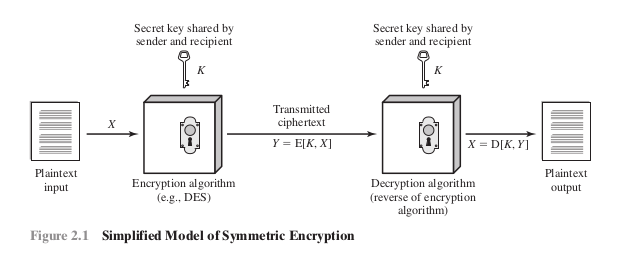
\includegraphics[width=14cm, keepaspectratio]{Bistarelli/img/cap_2/figura2.1.png}
\end{figure}

Uno schema di crittografia simmetrica ha cinque ingredienti (vedi Figura 2.1):
\begin{itemize}
    \item \textbf{Testo in chiaro:} Si tratta del messaggio o dei dati originali che vengono inseriti nell'algoritmo come in ingresso.
    
    \item \textbf{Algoritmo di crittografia:} L'algoritmo di crittografia esegue varie sostituzioni e trasformazioni sul testo in chiaro.
    
    \item \textbf{Chiave segreta:} La chiave segreta che è l'input dell'algoritmo di crittografia. 
    
    \item \textbf{Testo cifrato:} È il messaggio criptato prodotto in uscita. 
    
    Dipende dal testo in chiaro e dalla chiave segreta. Per un dato messaggio, due chiavi diverse produrranno due cifrari diversi.
    
   \item \textbf{Algoritmo di decifrazione:} Si tratta essenzialmente dell'algoritmo di crittografia eseguito  all'inverso. 
    
    Prende il testo cifrato e la chiave segreta e produce il testo in chiaro originale.
\end{itemize}
\newpage
I requisiti per un \textbf{uso sicuro della crittografia simmetrica} sono due:
\begin{enumerate}
    \item \textbf{È necessario un algoritmo di crittografia forte.}
    
   Se un avversario conosce l'algoritmo di cifratura ed ha accesso a uno o più testi cifrati non deve comunque essere in grado di decifrarli.
    
    \item \textbf{Il mittente e il destinatario devono aver ottenuto copie della chiave segreta in modo sicuro e devono mantenerla protetta.}
    
    Se qualcuno scopre la chiave e conosce l'algoritmo, tutte le comunicazioni che utilizzano la medesima chiave sono leggibili.
\end{enumerate}
Esistono due approcci generali per attaccare uno schema di crittografia simmetrica.
\paragraph{Il primo attacco} è noto come crittoanalisi. Gli attacchi di crittoanalisi si basano sulla natura dell'algoritmo e sulla conoscenza delle caratteristiche generali del testo in chiaro e del testo cifrato. 

\singlespacing

Questo tipo di attacco sfrutta le caratteristiche dell'algoritmo per cercare di dedurre un testo in chiaro specifico o di dedurre la chiave utilizzata. Se l'attacco riesce a dedurre la chiave, l'effetto è catastrofico: \textbf{Tutti i messaggi futuri e passati crittografati con quella chiave sono compromessi.}

\singlespacing

\paragraph{Il secondo metodo} noto come attacco a forza bruta, consiste nel provare ogni possibile chiave su un pezzo di testo cifrato finché non si ottiene una traduzione comprensibile in testo in chiaro. In media, la metà di tutte le chiavi possibili deve essere provata per ottenere un successo. Cioè, se ci sono x chiavi diverse, in media un attaccante scoprirebbe la chiave effettiva dopo $x/2$ tentativi.

\subsection{Algoritmi di crittografia a blocchi simmetrici}
Gli algoritmi di crittografia simmetrica più utilizzati sono \textbf{i cifrari a blocchi.} 

\singlespacing

Un cifrario a blocchi elabora il testo in chiaro in blocchi di dimensioni fisse e produce un blocco di testo cifrato di dimensioni uguali per ogni blocco di testo in chiaro. L'algoritmo elabora quantità di testo in chiaro come una serie di blocchi di dimensioni fisse. Gli algoritmi simmetrici più importanti, che sono tutti cifrari a blocchi, sono il Data Encryption Standard (DES), il triplo DES e l'Advanced Encryption Standard (AES)

\begin{figure}[H]
	\centering
    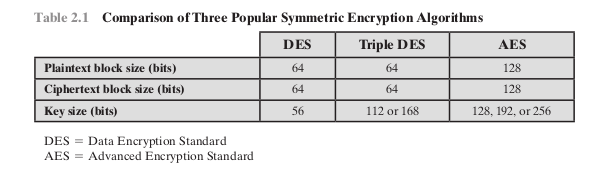
\includegraphics[width=14cm, keepaspectratio]{Bistarelli/img/cap_2/tabella2.1.png}
\end{figure}


Vedi tabella 2.1

\paragraph{DES} Fino a poco tempo fa, lo schema di crittografia più diffuso era basato sul Data Encryption Standard (DES). Il DES utilizza un blocco di testo in chiaro di 64 bit e una chiave di 56 bit per produrre un blocco di testo cifrato di 64 bit. I problemi del DES si dividono in due categorie: 

\begin{itemize}
    \item Problemi sull'algoritmo stesso
    
    \item Problemi sull'uso di una chiave a 56 bit. 
\end{itemize}
\paragraph{Il primo problema:} si riferisce alla possibilità che la crittoanalisi sia possibile sfruttando le caratteristiche dell'algoritmo DES. Nel corso degli anni, ci sono stati numerosi tentativi di trovare e sfruttare le debolezze dell'algoritmo, rendendo il DES l'algoritmo di crittografia più studiato in assoluto. Nonostante i numerosi approcci, finora nessuno ha segnalato una debolezza "cruciale" nel DES.

\singlespacing

\paragraph{IL secondo problema è la lunghezza della chiave.} Con una lunghezza di 56 bit, ci sono 256 chiavi possibili, pari a circa 7,2 * 1016 chiavi. Considerata la velocità dei processori in commercio, questa lunghezza di chiave è tristemente inadeguata. Un documento di Seagate Technology suggerisce che una velocità di un miliardo (109) di combinazioni di chiavi al secondo è ragionevole per gli attuali computer multicore. Le offerte recenti lo confermano. Sia Intel che AMD offrono ora istruzioni basate su hardware per accelerare l'uso di AES. I test condotti su una macchina Intel multicore contemporanea hanno dato come risultato una velocità di crittografia di circa mezzo miliardo di chiavi al secondo. Un'altra recente analisi suggerisce che, con la tecnologia contemporanea dei supercomputer, una velocità di 1013 crittografie/s è ragionevole.

\singlespacing

Tenendo conto di questi risultati, la Tabella 2.2 mostra quanto tempo è necessario per compiere un attacco di forza bruta per chiavi di varie dimensioni. Come si può notare, un singolo PC può violare il DES in circa un anno. Se più PC lavorano in parallelo, il tempo si riduce drasticamente. I supercomputer di oggi dovrebbero essere in grado di trovare una chiave in circa un'ora. Le chiavi di dimensioni 128 bit o superiori sono di fatto inviolabili con un semplice approccio di forza bruta. Anche se riuscissimo a velocizzare il sistema di attacco di un fattore di 1 trilione (1012), ci vorrebbero comunque più di 100.000 anni per decifrare un codice che utilizza una chiave a 128 bit. Fortunatamente esistono diverse alternative al DES, le più importanti delle quali sono il triplo DES e l'AES.

\singlespacing

\paragraph{TripleDes} La vita del DES è stata prolungata dall'uso del triple DES (3DES), che prevede \textbf{la ripetizione dell'algoritmo DES di base per tre volte} utilizzando due o tre chiavi uniche, per una dimensione della chiave di 112 o 168 bit. Il 3DES è stato standardizzato per la prima volta per l'uso in applicazioni finanziarie nello standard ANSI X9.17 nel 1985. Il 3DES ha due caratteristiche che ne assicurano la diffusione nei prossimi anni.

\begin{itemize}
    \item Grazie alla lunghezza della chiave di 168 bit, supera la vulnerabilità agli attacchi di forza bruta del DES.
    
    \item L'algoritmo di crittografia sottostante al 3DES è lo stesso del DES.
\end{itemize}

Questo algoritmo è stato sottoposto a maggiori controlli rispetto a qualsiasi altro algoritmo di crittografia per un periodo di tempo più lungo e non è stato trovato alcun attacco di crittoanalisi efficace basato sull'algoritmo piuttosto che sulla forza bruta. Di conseguenza, c'è un'elevato livello di fiducia che il 3DES sia molto resistente alla crittoanalisi.

\singlespacing

\textbf{Il principale svantaggio} del 3DES è che l'algoritmo è relativamente lento nel software. Il 3DES, che richiede un numero di calcoli tre volte i calcoli del DES, è di conseguenza più lento. Un altro svantaggio è che sia il DES che il 3DES utilizzano una dimensione di blocco di 64 bit. Per ragioni di efficienza e sicurezza, è auspicabile una dimensione di blocco maggiore.

\singlespacing

\paragraph{AES} A causa dei suoi svantaggi, il 3DES non è un candidato ottimale per un uso a lungo termine.
Per sostituirlo, nel 1997 il NIST ha pubblicato un invito a presentare proposte per un nuovo Advanced Encryption Standard (AES), che dovrebbe avere una forza di sicurezza pari o superiore al 3DES e un'efficienza sicurezza pari o superiore al 3DES ma sicuramente un'efficienza significativamente migliorata.

\singlespacing

Oltre a questi requisiti generali, il NIST ha specificato che AES deve essere un cifrario a blocchi simmetrico con un blocco simmetrico con una lunghezza di blocco di 128 bit e supporto per chiavi di 128, 192 e 256 bit. 
I criteri di valutazione includevano \textbf{la sicurezza, l'efficienza computazionale, requisiti di memoria, idoneità hardware e software e flessibilità.} In una prima fase di valutazione sono stati accettati 15 algoritmi proposti. In un secondo momento si è poi ristretto il campo a 5 algoritmi. Il NIST ha completato il processo di valutazione e ha pubblicato lo standard finale come FIPS PUB 197 (Advanced Encryption Standard, novembre 2001). 

\subsection{Cifrari a flusso}
Un cifrario a blocchi elabora l'input un blocco di elementi alla volta, producendo un blocco di output per ogni blocco di input. Un cifrario a flusso elabora gli elementi in ingresso in modo continuo, producendo un elemento in uscita alla volta, man mano che procede. Sebbene i cifrari a blocchi siano molto più comuni, ci sono alcune applicazioni in cui un cifrario a flusso è più appropriato. Un tipico cifrario a flusso cripta il testo in chiaro un byte alla volta, anche se un cifrario a flusso può essere progettato per operare su un bit alla volta o su unità di dimensioni piu' grandi di un byte alla volta.

\begin{figure}[H]
	\centering
    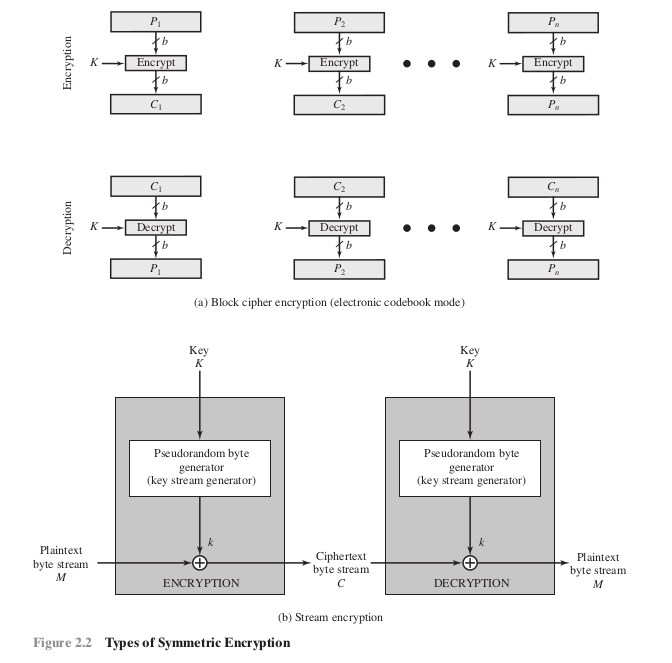
\includegraphics[width=14cm, keepaspectratio]{Bistarelli/img/cap_2/figura2.2.png}
\end{figure}

La Figura 2.2b è un diagramma rappresentativo della struttura di un cifrario a flusso. 

\singlespacing

In questa struttura, una chiave viene immessa in un generatore di bit pseudorandom che produce un flusso di numeri a 8 bit che sono apparentemente casuali. Un flusso pseudorandom è un flusso imprevedibile senza conoscere la chiave di ingresso e che ha un carattere apparentemente casuale. L'output del generatore, chiamato flusso di chiavi, viene combinato un byte alla volta con il flusso di testo in chiaro utilizzando l'operazione di OR esclusivo bitwise (XOR). Con un generatore di numeri pseudorandom correttamente progettato, un cifrario a flusso può essere sicuro quanto un cifrario a blocchi di lunghezza analoga. Il vantaggio principale di un cifrario a flusso è che i cifrari a flusso sono quasi sempre più veloci e utilizzano molto meno codice rispetto ai cifrari a blocco in piu' è possibile riutilizzare le chiavi. Per applicazioni che richiedono la crittografia/decrittografia di un flusso di dati, come ad esempio un canale di comunicazione dati o un browser/Web. Un cifrario a flusso potrebbe essere l'alternativa migliore. Per le applicazioni che trattano blocchi di dati, come il trasferimento di file, e-mail e database, i cifrari a blocchi possono essere più appropriati. Tuttavia, entrambi i tipi di di cifratura possono essere utilizzati praticamente in qualsiasi applicazione.
\section{Autenticazione basata su messaggio e funzioni Hash}
La crittografia protegge sia dagli \textbf{attacchi passivi} (intercettazioni) che dagli \textbf{attacchi attivi} (falsificazione di dati e transazioni). 

\singlespacing

La protezione contro tali attacchi è nota come autenticazione dei messaggi o dei dati. Un messaggio, un file, un documento o un'altra raccolta di dati si dice autentico quando è genuino e proviene dalla sua presunta fonte. L'autenticazione dei messaggi o dei dati è una procedura che consente alle parti comunicanti di verificare \textbf{che i messaggi ricevuti o memorizzati siano autentici.}

\singlespacing

I due aspetti importanti per l'autenticazione sono:

\begin{enumerate}
    \item Verificare che il contenuto del messaggio non sia stato alterato 
    
    \item La fonte deve essere autentica
\end{enumerate}

Si può anche voler verificare la tempestività di un messaggio (che non sia stato artificialmente ritardato e riprodotto) rispetto ad altri messaggi che scorrono tra due parti.

\subsection{Autenticazione usando la crittografia simmetrica}

Sembrerebbe possibile eseguire l'autenticazione semplicemente utilizzando la crittografia simmetrica. Se assumiamo che solo il mittente e il destinatario condividano una chiave (come dovrebbe essere), allora solo il mittente autentico sarebbe in grado di criptare con successo un messaggio per l'altro partecipante, a patto che il destinatario sia in grado di riconoscere un messaggio valido. 

\singlespacing

Inoltre, se il messaggio include un codice di rilevazione degli errori e un numero di sequenza, il destinatario ha la certezza che non sono state apportate alterazioni e che il che la sequenza è corretta. Se il messaggio include anche un timestamp, il destinatario è sicuro che il messaggio non è stato alterato e che la sequenza è corretta ed anche che il messaggio non ha subito ritardi superiori a quelli normalmente previsti per il transito in rete. 

\singlespacing

\textbf{In realtà, la crittografia simmetrica da sola non è uno strumento adatto per l'autenticazione dei dati.}

\singlespacing

Per fare un semplice esempio, nella modalità di crittografia BCE, se un aggressore riordina i blocchi di testo cifrato, ogni blocco verrà comunque decifrato con successo. Tuttavia, il riordino può alterare il significato della sequenza di dati complessiva. Anche se i numeri di sequenza possano essere utilizzati a un certo livello (ad esempio, ogni pacchetto IP), di solito non è il caso che un numero di sequenza separato sia associato a ciascun blocco b-bit di testo in chiaro.
Pertanto, il riordino dei blocchi è una minaccia.

\subsection{Autenticazione dei messaggi senza crittografia dei messaggi}
In tutti questi approcci, un tag di autenticazione viene generato e aggiunto a ogni messaggio per la trasmissione. Il messaggio stesso non è criptato e può essere letto a destinazione indipendentemente dalla funzione di autenticazione. Poiché gli approcci discussi in questa sezione non cifrano il messaggio e non garantiscono la riservatezza del messaggio. Come già detto, la crittografia dei messaggi di per sé come si è detto, non fornisce una forma sicura di autenticazione. Tuttavia, è possibile combinare l'autenticazione e la riservatezza in un unico algoritmo crittografando un messaggio e il suo tag di autenticazione. In genere, tuttavia, l'autenticazione dei messaggi viene fornita come una funzione separata dalla crittografia del messaggio e suggerisce tre situazioni in cui in cui l'autenticazione dei messaggi senza riservatezza è migliore:

\begin{itemize}
    \item Esistono diverse applicazioni in cui lo stesso messaggio viene trasmesso a più destinazioni.
    
Due esempi sono la notifica agli utenti che la rete non è più disponibile e la trasmissione di un messaggio a più destinazioni. Ovviamente è più economico e più affidabile avere una sola destinazione responsabile per il controllo dell'autenticità. Pertanto, il messaggio deve essere trasmesso in chiaro con un tag di autenticazione associato al messaggio. Il sistema responsabile esegue l'autenticazione. Se si verifica una violazione, gli altri sistemi di destinazione vengono avvisati da un allarme generale.

    \item Un altro scenario possibile è uno scambio in cui una parte ha un carico pesante e non può permettersi il tempo di decifrare tutti i messaggi in arrivo.

l'autenticazione viene effettuata in modo selettivo, scegliendo a caso i messaggi da controllare.

    \item L'autenticazione in chiaro è un servizio interessante. 
    
Il programma può essere eseguito senza doverlo decifrare ogni volta, che sarebbe uno spreco di risorse del processore. Tuttavia, se un'etichetta di autenticazione del messaggio al programma, questo potrebbe essere controllato ogni volta che si richiede una garanzia di dell'integrità del programma.
\end{itemize}
Pertanto, sia l'autenticazione che la crittografia possono essere utilizzate per soddisfare le esigenze di sicurezza.

\singlespacing

\paragraph{Codice di autenticazione del messaggio} E' una tecnica di autenticazione che prevede l'uso di una chiave segreta per generare un piccolo blocco di dati, noto come codice di autenticazione del messaggio, che viene aggiunto al messaggio. Questa tecnica presuppone che due parti comunicanti, ad esempio A e B, condividano una chiave segreta comune $K_{AB}$. Quando A ha un messaggio da inviare a messaggio da inviare a B, calcola il codice di autenticazione del messaggio come funzione complessa del messaggio e della chiave: $MAC_M = F(K_{AB}, M)$.3 Il messaggio più il codice vengono trasmessi al destinatario previsto. 

\singlespacing

Il destinatario esegue lo stesso calcolo sul messaggio ricevuto, utilizzando la stessa chiave segreta, per generare un nuovo codice di autenticazione del messaggio.
Il codice ricevuto viene confrontato con quello calcolato (cfr. Figura 2.3). Se assumiamo che solo il destinatario e il mittente conoscano l'identità della chiave segreta, e se il codice ricevuto corrisponde a quello calcolato, allora il codice ricevuto corrisponde al codice calcolato allora:

\begin{enumerate}
    \item Il destinatario ha la certezza che il messaggio non è stato alterato. Se un aggressore altera il messaggio ma non il codice, il calcolo del codice da parte del destinatario sarà diverso da quello ricevuto. Poiché si presume che l'aggressore non conosca la chiave segreta, l'aggressore non può alterare il codice in modo da far corrispondere alle alterazioni del messaggio.
    
    \item Il destinatario ha la certezza che il messaggio provenga dal presunto mittente. Poiché nessun altro conosce la chiave segreta, nessun altro potrebbe preparare un messaggio con un codice adeguato.

    \item  Se il messaggio include un numero di sequenza (come nel caso di X.25, HDLC e TCP), il destinatario può essere certo che il messaggio provenga dal presunto mittente perché un un aggressore non può alterare il numero di sequenza.

\end{enumerate}
Il DES o l'AES vengono utilizzati per generare una versione crittografata del messaggio, e alcuni di questi algoritmi vengono utilizzati per la creazione di un codice.

\begin{figure}[H]
	\centering
    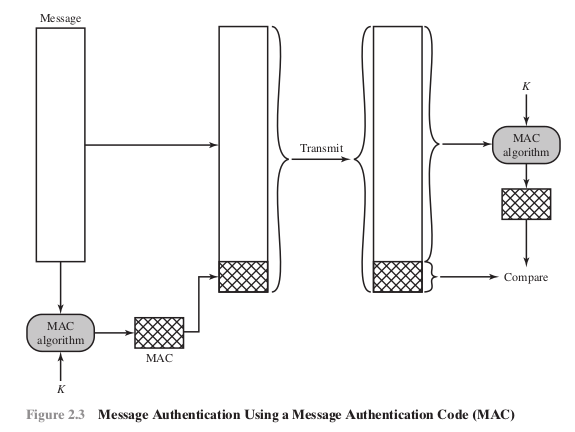
\includegraphics[width=14cm, keepaspectratio]{Bistarelli/img/cap_2/figura2.3.png}
\end{figure}

\paragraph{Funzione di hash a una via} Un'alternativa al codice di autenticazione dei messaggi è la funzione hash unidirezionale. Come nel caso del codice di autenticazione dei messaggi, una funzione di hash accetta in ingresso un messaggio M di dimensioni variabili e produce in uscita un digest del messaggio H(M) di dimensioni fisse (vedere Figura 2.4). In genere, il messaggio viene imbottito fino a un multiplo intero di una certa lunghezza fissa (ad esempio, 1024 bit) e l'imbottitura include il valore della lunghezza del messaggio originale in bit. Il campo della lunghezza è una misura di sicurezza per di sicurezza per aumentare la difficoltà per un aggressore di produrre un messaggio alternativo con lo stesso valore di hash.

\singlespacing

A differenza del MAC, una funzione di hash non riceve in ingresso una chiave segreta. La Figura 2.5 illustra tre modi in cui il messaggio può essere autenticato utilizzando una funzione hash.
Il digest del messaggio può essere crittografato utilizzando la crittografia simmetrica (vedere Figura 2.5a); se si presume che solo il mittente e il destinatario condividano la chiave di crittografia, l'autenticità è garantita.
Il message digest può anche essere crittografato con la crittografia a chiave pubblica (cfr. Figura 2.5b), come illustrato nella Sezione 2.3. L'approccio a chiave pubblica chiave pubblica presenta due vantaggi: 

\begin{enumerate}
    \item Fornisce una firma digitale
    
    \item L'autenticazione del messaggio e non richiede la distribuzione delle chiavi alle parti comunicanti
\end{enumerate}
Questi due approcci hanno un vantaggio rispetto a quelli che criptano l'intero messaggio, in quanto richiedono meno calcoli. Ma un approccio ancora più comune è l'uso di una tecnica che evita del tutto la crittografia. Diverse ragioni per questo interesse sono evidenziate in:

\begin{enumerate}
    \item \textbf{Il software di crittografia è piuttosto lento.}
    
    Anche se la quantità di dati da crittografia per ogni messaggio è piccola, può esserci un flusso costante di messaggi in entrata e in uscita da un sistema.

    \item \textbf{I costi dell'hardware di crittografia non sono trascurabili.} 
    
    Sono disponibili implementazioni su chip a basso costo di DES e AES, ma il costo aumenta se tutti i nodi di una rete devono avere questa capacità.
    
    \item \textbf{L'hardware di crittografia è ottimizzato per le grandi dimensioni dei dati.}
    
    Per piccoli blocchi di dati, un'alta percentuale del tempo viene spesa per l'overhead di inizializzazione/invocazione.
    
    \item \textbf{Un algoritmo di crittografia può essere protetto da un brevetto.}
\end{enumerate}

\begin{figure}[H]
	\centering
    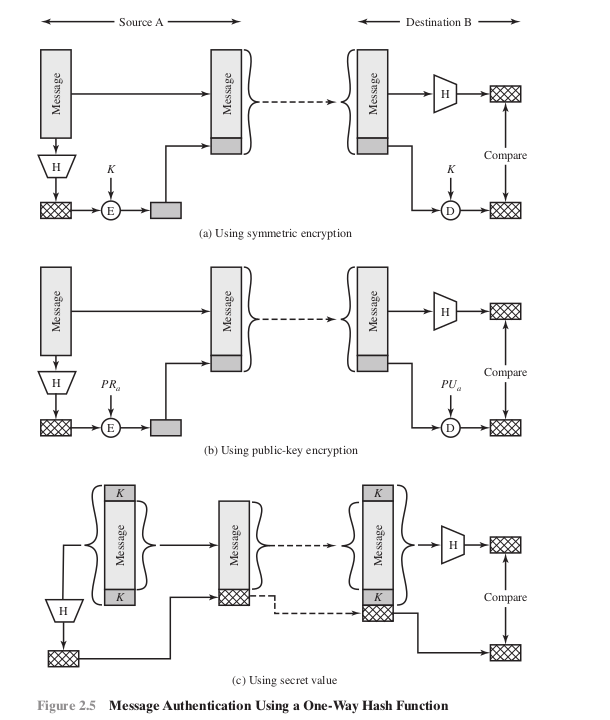
\includegraphics[width=14cm, keepaspectratio]{Bistarelli/img/cap_2/figura2.5.png}
\end{figure}


La Figura 2.5c mostra una tecnica che utilizza una funzione hash ma non la crittografia per l'autenticazione dei messaggi. Questa tecnica, nota come MAC hash a chiave, presuppone che due parti comunicanti, ad esempio A e B, condividano una chiave segreta comune K. Questa chiave segreta viene incorporata nel processo di generazione di un codice hash. Nell'approccio illustrato nella Figura 2.5c, quando A ha un messaggio da inviare a B, calcola la funzione di hash sulla concatenazione della chiave segreta e del messaggio: $M_{DM} = H(K || M || K)$. Quindi invia $[M  MD_{M}]$ a B. Poiché B possiede K, può ricalcolare $H(K ||  M ||  K)$ e verificare MDM. Dato che la chiave segreta non viene inviata, non dovrebbe essere possibile per un attaccante un aggressore di modificare un messaggio intercettato. Finché la chiave segreta rimane segreta, non dovrebbe essere possibile per un aggressore generare un messaggio falso.
Si noti che la chiave segreta viene utilizzata sia come prefisso che come suffisso del messaggio. Se la chiave segreta è usata solo come prefisso o solo come suffisso, lo schema è meno sicuro.

\newpage
\subsection{Altre applicazioni delle funzioni hash}
Ecco altri due esempi di applicazioni sicure delle funzioni hash:

\begin{itemize}
    \item \textbf{Password}
    
    In parole povere, quando un utente inserisce una password, l'hash di tale password viene confrontato con il valore di hash memorizzato per la verifica. Questa applicazione richiede resistenza alla preimmagine e forse una seconda resistenza alla preimmagine.
    
    \item \textbf{Rilevamento delle intrusioni}
    
    Memorizzare il valore di hash di un file, H(F), per ogni file su un sistema e proteggere i valori di hash (H(F)).
    Un sistema e proteggere i valori di hash (ad esempio, su un'unità bloccata in scrittura o su un disco ottico disco ottico write-once che viene tenuto al sicuro). È possibile determinare in seguito se un file è stato modificato calcolando nuovamente H(F). Un intruso dovrebbe modificare F senza modificare H(F).
\end{itemize}

\section{Crittografia a chiave pubblica}
\subsection{Struttura della crittografia a chiave pubblica}
Gli algoritmi a chiave pubblica sono basati su funzioni matematiche piuttosto che su semplici operazioni su schemi di bit, come quelle utilizzate negli algoritmi di crittografia simmetrica.  Inoltre, la crittografia a chiave pubblica è asimmetrica e prevede l'uso di due chiavi separate, a differenza della crittografia simmetrica che utilizza una sola chiave.

\singlespacing

L'uso di due chiavi ha profonde conseguenze nelle aree della riservatezza, della distribuzione delle chiavi e dell'autenticazione.

\singlespacing

Prima di procedere, è necessario menzionare alcune idee sbagliate comuni sulla crittografia a chiave pubblica. Una di queste è che la crittografia a chiave pubblica sia più sicura rispetto alla crittografia simmetrica. 
\singlespacing

In realtà, la sicurezza di qualsiasi schema di crittografia dipende da.

\begin{enumerate}

    \item \textbf{La lunghezza della chiave }
    
    \item \textbf{il lavoro computazionale necessario per di calcolo necessario per decifrare un cifrario}
\end{enumerate}

In linea di principio non c'è nulla nella crittografia simmetrica o della crittografia a chiave pubblica che ne renda una superiore all'altra dal punto di vista di resistenza agli attacchi. Una seconda convinzione errata è che la crittografia a chiave pubblica sia una tecnica di uso generale che ha reso obsoleta la crittografia simmetrica. Al contrario, a causa dell'overhead computazionale degli attuali schemi, non sembra che la crittografia simmetrica venga abbandonata.
Infine, si ha l'impressione che la distribuzione delle chiavi sia banale quando si usa la crittografia a chiave pubblica, rispetto a quella a chiave simmetrica. Per la distribuzione delle chiavi a chiave pubblica, è necessaria una qualche forma di protocollo, che spesso coinvolge un agente centrale, e le procedure non sono più semplici o più efficienti di quelle richieste per la crittografia simmetrica.

\singlespacing

Uno schema di crittografia a chiave pubblica ha sei ingredienti (vedi Figura 2.6a):

\begin{itemize}
    \item \textbf{Testo in chiaro}
    
    Si tratta del messaggio o dei dati leggibili che vengono inseriti nell'algoritmo come input.
    
    \item \textbf{Algoritmo di crittografia}
    
    L'algoritmo di crittografia esegue varie trasformazioni sul testo in chiaro.
    
    \item \textbf{Chiave Pubblica e Privata}
    
    Si tratta di una coppia di chiavi selezionate in modo che se una viene usata per la crittografia, l'altra viene usata per la decrittografia. Le trasformazioni esatte eseguite dall'algoritmo di crittografia dipendono dalla chiave pubblica o privata fornita in ingresso.
    
    \item \textbf{Testo cifrato}
    
    È il messaggio criptato prodotto in uscita. Dipende dal testo in chiaro e dalla chiave. Per un dato messaggio, due chiavi diverse produrranno due cifrari diversi.
    
    \item \textbf{Algoritmo di decrittazione}
    
    Questo algoritmo accetta il testo in chiaro e la chiave corrispondente e produce il testo in chiaro originale. 
\end{itemize}

Come suggeriscono i nomi, la chiave pubblica della coppia è resa pubblica e può essere utilizzata da altri, mentre la chiave privata è nota solo al suo proprietario. Un algoritmo crittografico di uso generale si basa su una chiave per la crittografia e su una chiave diversa ma correlata per la per la decifrazione.

\singlespacing

Le fasi essenziali sono le seguenti:

\begin{enumerate}

    \item Ogni utente genera una coppia di chiavi da utilizzare per la crittografia e la decrittografia dei messaggi.
    
    \item Ogni utente inserisce una delle due chiavi in un registro pubblico o in un altro file accessibile.
    
    \item Se Bob desidera inviare un messaggio privato ad Alice, Bob cripta il messaggio utilizzando la chiave pubblica di Alice.
    
    \item Quando Alice riceve il messaggio, lo decifra utilizzando la sua chiave privata. Nessun altro può decifrare il messaggio perché solo Alice conosce la chiave privata di Alice.
    
\end{enumerate}

\begin{figure}[H]
	\centering
    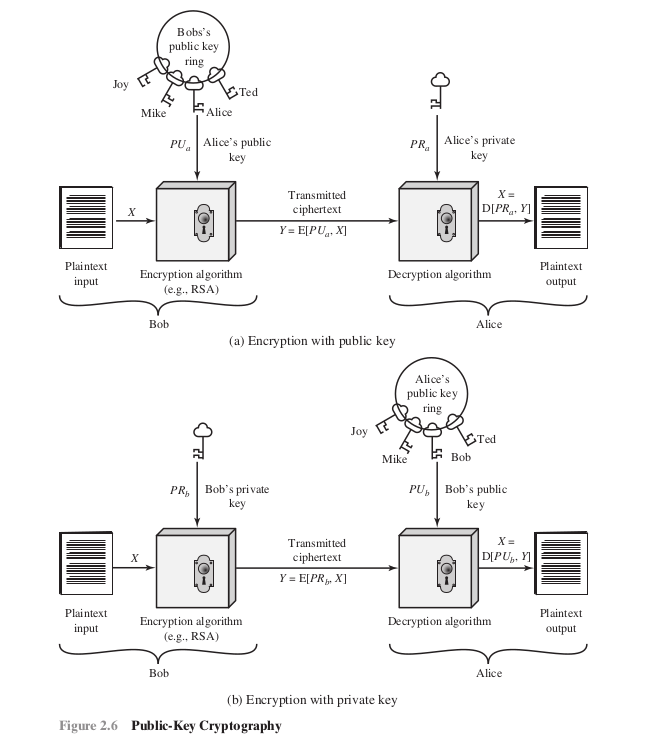
\includegraphics[width=14cm, keepaspectratio]{Bistarelli/img/cap_2/figura2.6.png}
\end{figure}

Con questo approccio, tutti i partecipanti hanno accesso alle chiavi pubbliche, mentre le chiavi private sono generate localmente da ogni partecipante e quindi non devono mai essere distribuite. Finché un utente protegge la propria chiave privata, la comunicazione in entrata è sicura. In qualsiasi momento, un utente può cambiare la chiave privata e pubblicare la nuova chiave pubblica che sostituisce la vecchia chiave pubblica.

\singlespacing

In questo schema, un utente cripta i dati utilizzando la propria chiave privata. Chiunque conosca la corrispondente chiave pubblica sarà in grado di decifrare il messaggio. Lo schema della Figura 2.6a è finalizzato a garantire la riservatezza. Solo il destinatario previsto deve essere in grado di decifrare il testo cifrato perché solo il destinatario previsto è in possesso di una chiave privata richiesta. 

\singlespacing

Lo schema della Figura 2.6b è finalizzato a fornire l'autenticazione e/o l'integrità dei dati. Se un utente è in grado di recuperare il testo in chiaro dal testo cifrato di Bob utilizzando la chiave pubblica di Bob, ciò indica che solo Bob può aver cifrato il testo in chiaro, fornendo così l'autenticazione. Inoltre, solo Bob sarebbe in grado di modificare il testo in chiaro perché solo Bob può cifrare il testo in chiaro con la chiave privata di Bob. 

\subsection{Applicazioni dei sistemi crittografici a chiave pubblica}
I sistemi a chiave pubblica sono caratterizzati dall'uso di un algoritmo di tipo crittografico con due chiavi, una privata e una pubblica. A seconda dell'applicazione, il mittente utilizza la chiave privata del mittente o la chiave pubblica del destinatario, o entrambe, per eseguire un tipo di funzione crittografica. In termini generali, possiamo classificare l'uso dei sistemi crittografici a chiave pubblica in tre categorie: firma digitale, distribuzione di chiavi simmetriche e crittografia di chiavi segrete.

\newpage
\subsection{Requisiti per la crittografia a chiave pubblica}
Il sistema crittografico illustrato nella Figura 2.6 dipende da un algoritmo crittografico
basato su due chiavi correlate. Diffie e Hellman hanno postulato questo sistema senza dimostrare l'esistenza di tali algoritmi.

\singlespacing

Tuttavia, hanno definito le condizioni che tali algoritmi devono soddisfare:

\begin{enumerate}
    \item È computazionalmente facile per una parte B generare una coppia (chiave pubblica $PU_b$, chiave privata $PR_b$).
    
    \item È computazionalmente facile per un mittente A, conoscendo la chiave pubblica e il messaggio da crittografare, M, per generare il corrispondente testo cifrato:
    
    \begin{center}
         $C = E(PU_b, M)$
    \end{center}
    
    \item È computazionalmente facile per il destinatario B decrittare il testo cifrato risultante utilizzando la chiave privata per recuperare il messaggio originale:
    
    \begin{center}
        $M = D(PR_b, C) = D[PR_b, E(PU_b, M)]$
    \end{center}
    
    \item È computazionalmente impossibile per un avversario, conoscendo la chiave pubblica, PUb, determinare la chiave privata, $PR_b$.
    
    \item  È computazionalmente impossibile per un avversario, conoscendo la chiave pubblica, PUb, e un testo cifrato, C, per recuperare il messaggio originale, M. Possiamo aggiungere un sesto requisito che, sebbene utile, non è necessario per tutte le applicazioni a chiave pubblica.
    
    \item Una delle due chiavi correlate può essere utilizzata per la crittografia e l'altra per la decrittografia.
    
    \begin{center}
        $M = D[PU_b, E(PR_b, M)] = D[PR_b, E(PU_b, M)]$
    \end{center}
\end{enumerate}

\begin{figure}[H]
	\centering
    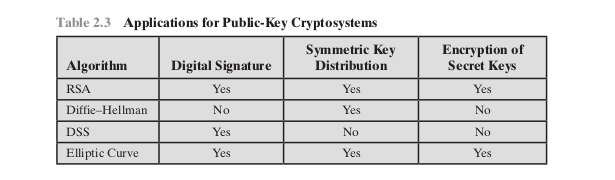
\includegraphics[width=14cm, keepaspectratio]{Bistarelli/img/cap_2/tabella2.3.png}
\end{figure}

\newpage
\subsection{Algoritmi di crittografia asimmetrica}
\paragraph{RSA} Lo schema RSA da allora regna sovrano come l'approccio alla crittografia a chiave pubblica. RSA è un cifrario a blocchi in cui il plaintext e il testo in chiaro e il testo cifrato sono numeri interi compresi tra 0 e $n - 1$ per qualche n. Per l'uso di RSA, è necessario utilizzare chiavi di dimensioni maggiori. Attualmente, una chiave di 1024 bit (circa 300 cifre decimali) è considerata abbastanza forte per quasi tutte le applicazioni.

\singlespacing

\paragraph{Accordo di chiave Diffie-Hellman} Il primo algoritmo a chiave pubblica pubblicato è apparso nell'articolo di Diffie e Hellman che ha definito la crittografia a chiave pubblica e viene generalmente chiamato scambio di chiavi Diffie-Hellman, o accordo di chiavi. Numerosi prodotti commerciali utilizzano questa tecnica di scambio di chiavi. Lo scopo dell'algoritmo è quello di permettere a due utenti di raggiungere in modo sicuro un accordo su un segreto condiviso che può essere usato come chiave segreta per la successiva crittografia simmetrica dei messaggi. L'algoritmo stesso si limita allo scambio delle chiavi.

\singlespacing


\paragraph{Standard di firma digitale} L'Istituto nazionale per gli standard e la tecnologia (NIST) ha pubblicato questo algoritmo come FIPS PUB 186 (Digital Signature Standard (DSS)). Il DSS fa uso di SHA-1 e presenta una nuova tecnica di firma digitale, l'algoritmo di firma digitale (DSA).  Il DSS utilizza un algoritmo progettato per fornire solo i dati di accesso al sistema. A differenza dell'RSA, non può essere utilizzato per la crittografia o lo scambio di chiavi.

\singlespacing

\paragraph{Crittografia a curva ellittica} La stragrande maggioranza dei prodotti e degli standard che utilizzano la crittografia a chiave pubblica per la crittografia e la firma digitale utilizzano RSA. La lunghezza dei bit per l'utilizzo sicuro di RSA è aumentata negli ultimi anni e ciò ha comportato un carico di elaborazione più pesante.
Questo ha comportato un carico di elaborazione maggiore per le applicazioni che utilizzano RSA. Recentemente, un sistema concorrente ha iniziato a sfidare RSA: la crittografia a curve ellittiche (ECC). L'ECC è già presente nelle iniziative di standardizzazione, tra cui l'IEEE (Istituto Elettrico). L'attrattiva principale dell'ECC rispetto all'RSA è che sembra offrire la stessa sicurezza per una dimensione di bit molto più piccola riducendo così l'overhead di elaborazione. D'altra parte, sebbene la teoria dell'ECC esista da tempo, è solo di recente che hanno cominciato ad apparire dei prodotti e che c'è stato un interesse crittoanalitico per la ricerca di punti deboli. Pertanto, il livello di fiducia nell'ECC non è ancora così alto come quello di RSA.
\newpage
\section{Firme digitali e gestione delle chiavi}
\subsection{Firme digitali}
La crittografia a chiave pubblica può essere utilizzata per l'autenticazione con una tecnica nota come firma digitale. Digital Signature Standard (DSS), definiscono la firma digitale come segue: Il risultato di una trasformazione crittografica di dati che, se correttamente implementata, fornisce un meccanismo per la verifica dell'origine l'autenticazione, l'integrità dei dati e il non ripudio del firmatario. Pertanto, una firma digitale è un modello di bit dipendente dai dati, generato da un agente in funzione di un file, di un messaggio o di un'altra forma di blocco di dati. 

\singlespacing

Il FIPS 186-4 specifica l'uso di uno dei tre algoritmi di firma digitale:
\begin{itemize}
    \item Algoritmo di firma digitale (DSA): L'algoritmo originale approvato dal NIST, che si basa sulla difficoltà di calcolo dei logaritmi discreti.
    
    \item Algoritmo di firma digitale RSA: Basato sull'algoritmo a chiave pubblica RSA.
    
    \item Algoritmo di firma digitale a curva ellittica (ECDSA): basato sulla crittografia a curva ellittica.
\end{itemize}

\begin{figure}[H]
	\centering
    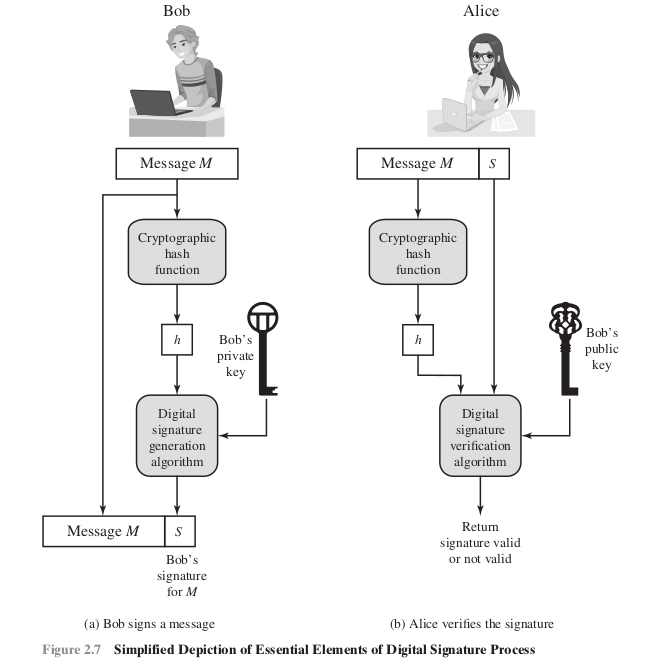
\includegraphics[width=14cm, keepaspectratio]{Bistarelli/img/cap_2/figura2.7.png}
\end{figure}


La Figura 2.7 è un modello generico del processo di creazione e utilizzo delle firme digitali. Tutti gli schemi di firma digitale previsti dal FIPS 186-4 hanno questa struttura. Supponiamo che Bob voglia inviare un messaggio ad Alice. Sebbene non sia importante che il messaggio segreto, Bob vuole che Alice abbia la certezza che il messaggio provenga da lui. A tal fine, Bob utilizza una funzione di hash sicura, come SHA-512, per generare un valore di hash per il messaggio. Questo valore di hash, insieme alla chiave privata di Bob, serve come input per un algoritmo di generazione della firma digitale che produce un breve blocco che funge da firma digitale. Bob invia il messaggio con la firma allegata.

\singlespacing

Quando Alice riceve il messaggio e la firma:

\begin{enumerate}
    \item calcola un valore di hash per il messaggio
    
    \item fornisce il valore di hash per il messaggio e la chiave pubblica di Bob come input a un algoritmo di verifica della firma digitale.
\end{enumerate}

Se l'algoritmo restituisce il risultato che la firma è valida, Alice ha la certezza che il messaggio è stato firmato da Bob. Nessun altro possiede la chiave privata di Bob e quindi nessun altro può aver creato una firma che possa essere verificata per questo messaggio con la chiave pubblica di Bob. Inoltre, è impossibile alterare il messaggio senza accedere alla chiave privata di Bob, quindi il messaggio è autenticato sia in termini di origine che di integrità dei dati. La firma digitale non garantisce la riservatezza. Cioè, il messaggio inviato  è al sicuro da alterazioni, ma non da intercettazioni. Questo è evidente nel caso di una firma basata su una parte del messaggio, perché il resto del messaggio viene trasmesso in chiaro. Anche nel caso di una crittografia completa, non c'è alcuna protezione della riservatezza, perché qualsiasi osservatore può decifrare il messaggio utilizzando la chiave pubblica del mittente. 

\subsection{Certificati a chiave pubblica}
Esiste un algoritmo a chiave pubblica ampiamente accettato, come RSA, ogni partecipante può inviare la propria chiave pubblica a qualsiasi altro partecipante o trasmettere la chiave alla comunità in generale. Sebbene questo approccio sia conveniente, ha una grande debolezza. Chiunque può falsificare tale annuncio pubblico. Cioè, un utente potrebbe fingere di essere Bob e inviare una chiave pubblica a un altro partecipante o trasmettere tale chiave pubblica. Finché Bob non scopre la falsificazione e avvisa gli altri partecipanti, il falsario è in grado di leggere tutti i messaggi cifrati destinati a Bob e può utilizzare le chiavi falsificate per l'autenticazione.

\singlespacing

\begin{figure}[H]
	\centering
    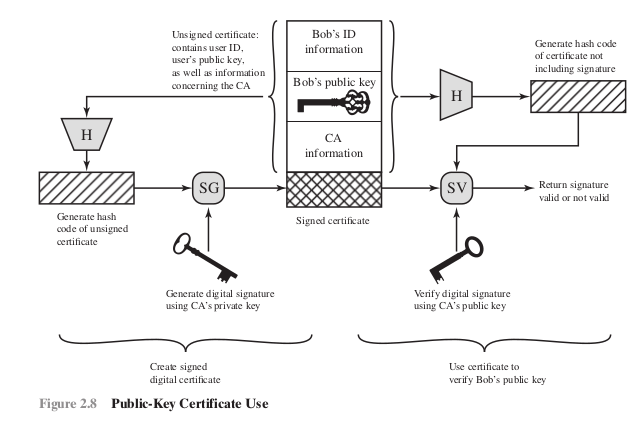
\includegraphics[width=14cm, keepaspectratio]{Bistarelli/img/cap_2/figura2.8.png}
\end{figure}

\textbf{La soluzione} a questo problema è il certificato a chiave pubblica. In sostanza, un certificato è costituito da una chiave pubblica più un ID utente del proprietario della chiave, con l'intero blocco firmato da una terza parte fidata. Il certificato include anche alcune informazioni sulla terza parte e un'indicazione del periodo di validità del certificato. In genere, la terza parte è un'autorità di certificazione (CA) di cui si fida la comunità degli utenti, come un'agenzia governativa o un'istituzione finanziaria. Un utente può presentare la propria chiave pubblica all'autorità in modo sicuro e ottenere un certificato firmato. L'utente può quindi pubblicare il certificato. Chiunque abbia bisogno della chiave pubblica di questo utente può ottenere il certificato e verificarne la validità attraverso la firma di fiducia allegata. La Figura 2.8 illustra il processo. Le fasi principali possono essere riassunte come segue:

\begin{enumerate}
    \item Il software utente (client) crea una coppia di chiavi: una pubblica e una privata.
    
    \item Il client prepara un certificato non firmato che include l'ID utente e la chiave pubblica dell'utente.
    
    \item L'utente fornisce il certificato non firmato a una CA in modo sicuro. Questo potrebbe un incontro faccia a faccia, l'uso di un'e-mail registrata o un modulo Web con verifica via e-mail.
    
    \item La CA crea una firma come segue:
        
        \begin{itemize}
            \item La CA utilizza una funzione hash per calcolare il codice hash del certificato non firmato.
            
            Una funzione di hash è una funzione che mappa un blocco di dati o un messaggio di lunghezza variabile in un valore di lunghezza fissa, chiamato codice hash.
            
            \item La CA genera la firma digitale utilizzando la chiave privata della CA e un algoritmo di generazione della firma.
            
        \end{itemize}
    
    \item La CA appone la firma al certificato non firmato per creare un certificato firmato.
    
    \item La CA restituisce al cliente il certificato firmato.
    
    \item Ogni utente può verificare la validità del certificato come segue:
        
        \begin{itemize}
            \item L'utente calcola il codice hash del certificato (esclusa la firma).
            
            \item L'utente verifica la firma digitale utilizzando la chiave pubblica della CA e l'algoritmo di verifica della firma. L'algoritmo restituisce un risultato di firma valida o non valida.
        \end{itemize}

\end{enumerate}
Uno schema è diventato universalmente accettato per la formattazione dei certificati a chiave pubblica, lo standard X.509. I certificati X.509 sono utilizzati nella maggior parte delle applicazioni per la sicurezza di rete, tra cui applicazioni di sicurezza di rete, tra cui IP Security (IPsec), Transport Layer Security (TLS), Secure Shell (SSH) e Secure Shell e Secure/Multipurpose Internet Mail Extension (S/MIME). La maggior parte di queste esamineremo la maggior parte di queste applicazioni nella quinta parte.

\subsection{Scambio di chiavi simmetriche con crittografia a chiave pubblica}
Con la crittografia simmetrica, un requisito fondamentale affinché due parti possano comunicare in modo sicuro è la condivisione di una chiave segreta. Supponiamo che Bob voglia creare un'applicazione di messaggistica che gli consenta di scambiare e-mail in modo sicuro con chiunque abbia accesso a Internet o a un'altra rete condivisa da entrambi. Supponiamo che Bob voglia farlo utilizzando la crittografia simmetrica. Con la crittografia simmetrica, Bob e la sua corrispondente, diciamo Alice, devono trovare un modo per condividere una chiave segreta unica che nessun altro conosce. Come possono farlo? Se Alice si trova nella stanza accanto a Bob, quest'ultimo potrebbe generare una chiave e scriverla su un foglio di carta o memorizzarla su un disco o una chiavetta e consegnarla ad Alice. Ma se Alice si trova dall'altra parte del continente o del mondo, cosa può fare Bob? Potrebbe criptare la chiave con la crittografia simmetrica e inviarla via e-mail ad Alice, ma ciò significa che Bob e Alice devono condividere una chiave segreta per criptare la nuova chiave segreta. Inoltre, Bob e chiunque altro utilizzi questo nuovo pacchetto di e-mail si trova ad affrontare lo stesso problema con ogni potenziale corrispondente: Ogni coppia di corrispondenti deve condividere una chiave segreta unica. Un approccio è l'uso dello scambio di chiavi Diffie-Hellman. Questo approccio è in effetti ampiamente utilizzato. Tuttavia, soffre dell'inconveniente che, nella sua forma più semplice, Diffie-Hellman non prevede l'autenticazione dei due interlocutori. Esistono esistono varianti di Diffie-Hellman che superano questo problema. Inoltre, esistono protocolli che utilizzano altri algoritmi a chiave pubblica che raggiungono lo stesso obiettivo.
\subsection{Buste Digitali}

\begin{figure}[H]
	\centering
    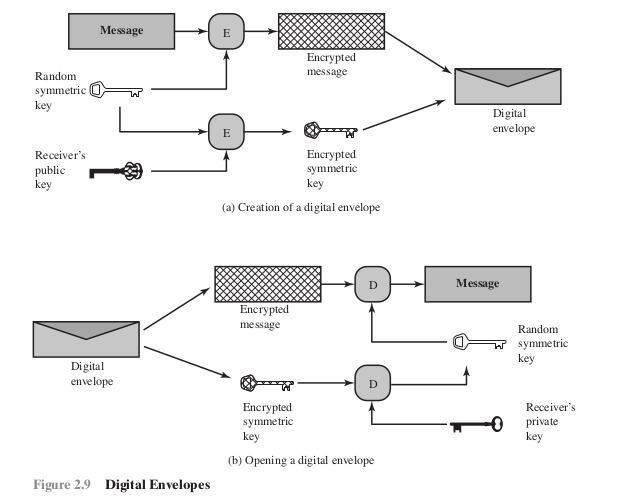
\includegraphics[width=14cm, keepaspectratio]{Bistarelli/img/cap_2/figura2.9.png}
\end{figure}


Un'altra applicazione in cui la crittografia a chiave pubblica viene utilizzata per proteggere una chiave simmetrica è la busta digitale, che può essere usata per proteggere un messaggio senza dover prima fare in modo che mittente e destinatario abbiano la stessa chiave segreta. La tecnica è denominata busta digitale, che è l'equivalente di una busta sigillata contenente una lettera non firmata. L'approccio generale è illustrato nella Figura 2.9. Supponiamo che Bob voglia inviare un messaggio riservato ad Alice, ma che non condivida una chiave segreta simmetrica. 

\singlespacing

Bob esegue le seguenti operazioni:

\begin{enumerate}

    \item Preparare un messaggio.
    
    \item Generare una chiave simmetrica casuale che verrà utilizzata una sola volta.
    
    \item Crittografare il messaggio utilizzando la crittografia simmetrica della chiave unica.
     
    \item Crittografare la chiave una tantum utilizzando la crittografia a chiave pubblica con la chiave pubblica di Alice.
    
    \item Allegare la chiave monouso crittografata al messaggio crittografato e inviarlo ad Alice.
    
\end{enumerate}
Solo Alice è in grado di decifrare la chiave a tempo unico e quindi di recuperare il messaggio originale. Se Bob ha ottenuto la chiave pubblica di Alice per mezzo del certificato di certificato a chiave pubblica di Alice, Bob ha la certezza che si tratta di una chiave valida.
\section{Applicazione pratica: Crittografia dei dati memorizzati}
Uno dei principali requisiti di sicurezza di un sistema informatico è la protezione dei dati memorizzati. I meccanismi di sicurezza per garantire tale protezione includono il controllo degli accessi, di rilevamento delle intrusioni e schemi di prevenzione delle intrusioni. Ma oltre agli approcci tecnici, questi approcci possono diventare vulnerabili a causa di fattori umani. Ne elenchiamo qui alcuni esempi, basati su:
\begin{itemize}
    \item Nel dicembre 2004, alcuni dipendenti della Bank of America hanno eseguito il backup e poi inviato al proprio centro dati di backup nastri contenenti i nomi dei clienti, gli indirizzi, i numeri di conto corrente e i numeri di previdenza sociale di 1,2 milioni di lavoratori pubblici iscritti a un conto con carta di credito. Nessuno dei dati era criptato. 
    
    I nastri non sono mai arrivati e non sono mai stati ritrovati. Purtroppo, questo metodo di backup e spedizione dei dati è fin troppo comune. Per fare un altro esempio, nell'aprile del 2005 Ameritrade ha incolpato il suo fornitore di spedizioni per aver perso un nastro di backup contenente informazioni non crittografate su 200.000 clienti.
    
    \item Nell'aprile del 2005, il San Jose Medical Group ha annunciato che qualcuno aveva fisicamente rubato uno dei suoi computer e un'altra parte di esso.
    
    \item Ci sono stati innumerevoli esempi di computer portatili persi negli aeroporti, rubati da una auto parcheggiata o presi mentre l'utente è lontano dalla sua scrivania. Se i dati sul disco non sono criptati, tutti i dati sono a disposizione del ladro.
\end{itemize}
Finché l'utente protegge la propria e non usa una password facilmente indovinabile, i file sono completamente protetti a protetti quando sono a riposo. 

\singlespacing

Alcuni approcci più recenti sono elencati in:

\begin{itemize}
    \item \textbf{Dispositivo back-end}
    
    Si tratta di un dispositivo hardware che si colloca tra i server e i sistemi di archiviazione e cripta tutti i file. Questi dispositivi criptano i dati a una velocità alla velocità del cavo, con una latenza molto ridotta. Al contrario, il software di crittografia sui server e sui sistemi di archiviazione rallenta i backup. 
    
    \item \textbf{Crittografia dei nastri basata su libreria}
    
    È fornita da una scheda co-processore incorporata nell'unità nastro e integrato nell'unità nastro e nell'hardware della libreria a nastro. Il co-processore cripta i dati utilizzando una chiave non leggibile configurata nella scheda. I nastri possono essere inviati fuori sede a una struttura che dispone dello stesso hardware dell'unità a nastro. La chiave può essere esportata tramite un' e-mail sicura o una piccola unità flash che viene trasportata in modo sicuro. 
    
    \item \textbf{Crittografia di base dei dati di laptop e PC}
    
    Diversi fornitori offrono prodotti prodotti software che forniscono una crittografia trasparente all'applicazione e all'utente. Alcuni prodotti crittografano tutti i file e le cartelle o una parte di essi. Altri prodotti, come altri prodotti, come BitLocker di Windows e FileVault di MacOS, crittografano un intero disco o un'immagine del disco o un'immagine del disco che si trova sul disco rigido dell'utente o su un dispositivo di archiviazione di rete.
\end{itemize}
